\documentclass[11pt,a4paper]{article}

% ---------------------------------------------------------------------------
% Objective 4 report: targeted adaptation with LoRA
% Compile with:  pdflatex objective4_report.tex  (run twice for references)
% Figures are expected in ./figs/ (produced by make_figs.py).
% ---------------------------------------------------------------------------

\usepackage[margin=2.4cm]{geometry}
\usepackage[T1]{fontenc}
\usepackage{mathpazo}
\usepackage{microtype}
\usepackage{graphicx}
\usepackage{booktabs}
\usepackage{tabularx}
\usepackage{xltabular}
\usepackage{array}
\usepackage{multirow}
\usepackage{xcolor}
\usepackage{enumitem}
\usepackage{amsmath,amssymb}
\usepackage{caption}
\usepackage{float}
\usepackage{tikz}
\usetikzlibrary{arrows.meta,positioning,shapes.geometric,fit,calc}
\usepackage[hidelinks]{hyperref}

\definecolor{ink}{HTML}{0B0B0B}
\definecolor{ink2}{HTML}{52514E}
\definecolor{qblue}{HTML}{2A78D6}
\definecolor{qorange}{HTML}{EB6834}
\definecolor{qaqua}{HTML}{1BAF7A}
\definecolor{qred}{HTML}{C9302C}
\definecolor{boxfill}{HTML}{F3F7FD}
\definecolor{fixfill}{HTML}{EEF7EE}

\captionsetup{font=small,labelfont=bf}
\setlist{itemsep=2pt,topsep=4pt}
\renewcommand{\arraystretch}{1.18}
\newcolumntype{L}{>{\raggedright\arraybackslash}X}
\newcommand{\met}{\textcolor{qaqua}{\textbf{met}}}
\newcommand{\missed}{\textcolor{qred}{\textbf{missed}}}
\newcommand{\na}{\textcolor{ink2}{n/a}}

% Placeholder: replace before submission
\newcommand{\placeholder}[1]{\textcolor{red}{[#1]}}
\newcommand{\reportdate}{29 October 2026}


\title{\textbf{Teaching a Small Kiosk Model the Behaviour\\the Harness Could Only Patch}\\[4pt]
\large Objective 4: Targeted Adaptation with LoRA}
\author{Anany Dev Choudhary\\\small Roll No.\ 228070135\\\small Department of Electrical Engineering\\\small Indian
Institute of Technology Kanpur}
\date{\reportdate}

\begin{document}
\maketitle

\begin{abstract}
\noindent
Objective~3 built a harness around two fixed small models for an offline watch-store kiosk, Qwen3.5-2B on a CPU-only
tier (A) and Qwen3.5-4B on an integrated-GPU tier (B). Several of its gains rest on patches that catch the models'
mistakes after the fact: tool calls printed as text, needless staff calls, values stated for fields the store does not
list, weak declines, and a 4B that breaks its tool-call format when asked for short replies. Objective~4 trains that
behaviour into the models instead, with small low-rank (LoRA) adapters loaded at run time next to the unchanged deployed
model files, while facts stay in retrieval. The training data comes from a second fictional catalogue that shares no
name or code with the store, so the models learn behaviour, not facts. Code decides every correct action; a
larger open model writes the replies, which pass automatic checks and a hand review. Every rule was fixed before its
run, and this round is a prototype on fictional data: it is judged on development data only, and the final training and
test set wait for the company's data.
On dev, the 2B adapter answers \textbf{83.0\% of store questions against 71.1\%} (+11.9 points), declines correctly on
\textbf{97.4\% of unanswerable and near-miss questions against 61.5\%}, makes no staff calls on answerable questions
(20 before) and prints no tool calls; nothing is worse. The 4B adapter is a tie on every set but lets the 4B keep its
short-reply rule, which without the adapter costs 9 points on store questions and prints 27 tool calls. With the
adapters, O3-final's behavioural patches can be switched off for both tiers. The deployment rule for Tier~A then fails
on speed: with the patches off, tool-case replies on the laptop CPU take 2.65\,s longer, so Tier~A keeps O3-final and
the adapter's gain is reported with its cost; the same adapter with the patches on was faster on both sets. Tier~B
deploys the 4B adapter with short replies and the patches off. The adapters also decline a few answerable policy and care
questions and some colour follow-ups they used to answer, a cost to fix in the data before the final round.
\end{abstract}

\tableofcontents
\vspace{6pt}
\hrule

% ===========================================================================
\section{Introduction}\label{sec:intro}
% ===========================================================================

\subsection{Where Objective 3 left the assistant}
The assistant answers customers at an in-store kiosk of a fictional watch retailer, entirely offline. Objective~3
confirmed a deployed setup, \textbf{O3-final}, in which an intent router sends each message down the cheapest path, the
kiosk runs most tool calls itself, and checks guard the knowledge path. On the test set the 2B rose from 51.9\% to 69.6\%
on store questions and the 4B from 66.7\% to 90.0\% on follow-ups. What remained was behaviour of the models themselves,
held in place on dev only by patches (Table~\ref{tab:gaps}). A blind judge also found unsupported claims in 23\% (4B)
and 37\% (2B) of replies to unanswerable questions.

\begin{table}[H]
\centering\small
\caption{The gaps Objective~4 targets, from Objective~3's dev results, and the patch that held each in place.}
\label{tab:gaps}
\begin{tabularx}{\textwidth}{L p{1.0cm} p{4.6cm}}
\toprule
Gap (dev evidence) & Tier & Patch in O3-final \\
\midrule
Tool call written as text instead of an answer (2B: 109 of 151 store questions in O3 Step~5; 4B under the short-reply
rule: 14) & both & forced-answer recovery, then a fixed staff line \\
Staff called on answerable questions (2B: 20--28 of 96) & A & staff check, which rarely changed the outcome \\
Values stated for fields the card lists as ``not listed'' & both & answer check (catches some) \\
Weak declines on unanswerable and near-miss questions (2B: 61--64\%) & A & entity check, hard fallback \\
Wrong tool choice (2B: tool selection 66.7\%, refusal 62.5\%) & A & routing by the kiosk \\
Cannot follow a reply-length rule without breaking the tool-call format & B & short-reply rule dropped, so its speed
gain is lost \\
\bottomrule
\end{tabularx}
\end{table}

\subsection{Objective 4}
Objective~4 trains the behaviour the harness can only patch, not the facts: facts change with the catalogue and stay in
retrieval. The same two models are adapted with LoRA adapters~\cite{lora}, one per tier, on the language layers only, and
the adapter is loaded at run time next to the deployed GGUF file, so the deployed weights stay byte-identical (route~(a)).
One QLoRA adapter~\cite{qlora} on the 2B is compared with LoRA. The company's data is not yet available, so this round
builds and tests the whole path on fictional data; the final training, the merged-weights route~(b) and a fresh test set
wait for that data.

\subsection{Hypotheses}
Each was written before any training run.
\begin{itemize}
  \item \textbf{H1, format.} With the adapter, printed tool calls fall to at most one per set for both models, including the
        4B with the short-reply rule.
  \item \textbf{H2, staff discipline (Tier~A).} The 2B's staff calls on answerable store questions at least halve, with
        answerable questions not worse.
  \item \textbf{H3, honest declines (Tier~A).} The 2B's unanswerable and near-miss questions improve by at least 5 points,
        and unsupported replies do not rise.
  \item \textbf{H4, no regression.} No set is worse for either model; Hinglish does not fall by more than 5 points.
  \item \textbf{H5, fewer patches.} With the adapter, O3-final's behavioural patches can be switched off without any set
        becoming worse; for the 4B this would recover the short replies and their speed.
  \item \textbf{H6, LoRA against QLoRA.} On the 2B, QLoRA is not better than LoRA (the model's fine-tuning guide advises
        against 4-bit QLoRA for this family).
\end{itemize}
Expected overall: larger gains for the 2B, which has the most room; for the 4B, mainly H5. The main risk is that training
on one catalogue's style narrows behaviour elsewhere; H4 and the Hinglish check guard against it.

\subsection{Structure of this report}
Section~\ref{sec:criteria} gives the rules, Section~\ref{sec:method} the method step by step, and
Section~\ref{sec:results} the dev comparison, the patch removal and the in-place speed test. Sections~\ref{sec:decisions}
to~\ref{sec:next} record decisions, limitations and what the final round must do.

% ===========================================================================
\section{Success criteria}\label{sec:criteria}
% ===========================================================================
All criteria compare O3-final with an adapter against O3-final itself, per tier, on the development data, with Objective~3's
verdict rule: a set is better or worse only if the paired bootstrap 95\% interval~\cite{efron} excludes zero and the
difference exceeds the noise bound of repeated greedy runs. Table~\ref{tab:criteria} gives them.

\begin{table}[H]
\centering\small
\caption{Success criteria, fixed before any run.}\label{tab:criteria}
\begin{tabularx}{\textwidth}{p{4.2cm} L}
\toprule
Criterion & Rule \\
\midrule
Keep an adapter & H4 holds, and at least one of H1 (as a gain), H2, H3 holds for that tier \\
Format (H1) & at most 1 printed tool call in each set; a gain only if O3-final printed more than 1 somewhere \\
Staff discipline (H2, 2B) & staff calls on answerable questions at most half, answerable not worse; testable if O3-final
made at least 4 \\
Declines (H3, 2B) & unanswerable and near-miss +5 points with the interval excluding 0; unsupported rate not higher \\
No regression (H4) & no single-turn set worse; dialogues meet Objective~3's targets with fit not lower; Hinglish, pooled over
the three single-turn sets (46 cases), within 5 points \\
Patches removed (H5) & adapter without patches: no regression against O3-final, and printed calls within H1 \\
Speed (Tier~A, in place) & (1) the adapter keeps at least 90\% of O3-final's writing speed; (2) the deployed candidate's
median total reply time is not significantly longer, on store questions and on tool cases \\
LoRA vs QLoRA (H6) & reported; QLoRA carried only if LoRA is not kept and QLoRA is not worse on any set \\
\bottomrule
\end{tabularx}
\end{table}

% ===========================================================================
\section{Method}\label{sec:method}
% ===========================================================================

\subsection{Protocol}
As in Objective~3, each step's rule was written into the project's objectives document before its run, and any
deviation is stated where it happened. The harness, scorers and timing are Objective~3's, unchanged. Quality runs use the
laptop's integrated GPU (Vulkan) for both models; the decisive timing for Tier~A is measured in place on the laptop CPU.
GPU work (teacher replies and training) ran on cloud T4 GPUs within a 20-hour weekly budget, and CPU-only work such as
adapter conversion ran in a cloud notebook. The harness, data generators, filters and analysis scripts were written for
this project; an AI coding assistant helped write and debug parts of this code.

\begin{figure}[H]
\centering
\resizebox{\textwidth}{!}{%
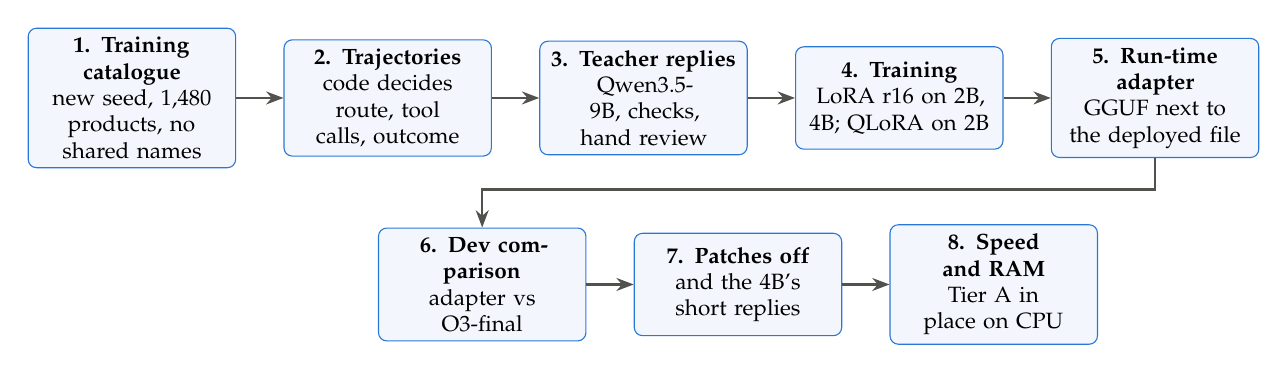
\begin{tikzpicture}[
  node distance=5mm and 6mm,
  box/.style={draw=qblue, fill=boxfill, rounded corners=3pt, align=center, font=\footnotesize, minimum height=13mm,
              text width=24mm},
  arr/.style={-{Stealth[length=2.2mm]}, thick, ink2}]
\node[box] (cat) {\textbf{1. Training catalogue}\\new seed, 1,480 products, no shared names};
\node[box, right=of cat] (traj) {\textbf{2. Trajectories}\\code decides route, tool calls, outcome};
\node[box, right=of traj] (teach) {\textbf{3. Teacher replies}\\Qwen3.5-9B, checks, hand review};
\node[box, right=of teach] (train) {\textbf{4. Training}\\LoRA r16 on 2B, 4B; QLoRA on 2B};
\node[box, right=of train] (gguf) {\textbf{5. Run-time adapter}\\GGUF next to the deployed file};
\node[box, below=9mm of traj, xshift=12mm] (s6) {\textbf{6. Dev comparison}\\adapter vs O3-final};
\node[box, right=of s6] (s7) {\textbf{7. Patches off}\\and the 4B's short replies};
\node[box, right=of s7] (s8) {\textbf{8. Speed and RAM}\\Tier~A in place on CPU};
\draw[arr] (cat) -- (traj); \draw[arr] (traj) -- (teach); \draw[arr] (teach) -- (train); \draw[arr] (train) -- (gguf);
\draw[arr] (gguf.south) |- ++(0,-4mm) -| (s6.north);
\draw[arr] (s6) -- (s7); \draw[arr] (s7) -- (s8);
\end{tikzpicture}}
\caption{The eight steps of Objective~4. Steps~1--5 build the adapters; Steps~6--8 decide them on dev data.}
\label{fig:steps}
\end{figure}

\subsection{Step 1: a training catalogue}
The deployed catalogue generator was run with a new seed. The training catalogue has 59 collections, 651 designs, 1,480
products and an 812-chunk store-knowledge corpus. Every collection is renamed, design codes start at V6000 (the deployed
range is V1001--V4258), store names and hours are new, service prices are scaled by 1.2 and service times moved by a few
days. A check confirms that no collection name, style name or product code is shared with the deployed catalogue, and that
the deployed catalogue still regenerates byte for byte. The adapter therefore cannot learn the store's facts; it can only
learn to answer from what it is shown.

\subsection{Step 2: trajectories decided by code}
For each target behaviour, questions were generated on the training catalogue: Objective~3's evaluation generators re-run
with new seeds, plus new templates for ``not listed'' attributes, unlisted policies, made-up designs, refusals and follow-up
wording. An \emph{oracle} stands in for the model behind the real harness, running O3-final's settings per tier, and gives
the correct next action for every request (answer, decline, call staff, ask, or a tool call). A product fact counts as
shown only on that product's own card or tool result. Because the harness itself builds each request, the training text
is exactly what the model sees at run time: system prompt, tool schemas, focused cards, thinking off.

Leakage was controlled by dropping any question that copies an evaluation question in any split, including Objective~3's
test set, or overlaps one by word Jaccard $\ge 0.6$; 897 generated questions were dropped. The final mix, built with the
deployed retrieval, has 3,000 examples per tier from 2,863 questions, 31\% of them Hinglish (Figure~\ref{fig:data}). Two
target shares miss their 10\% floor and were disclosed rather than topped up: declines (9.4\%), because the harness's own
entity check and fallback answer most made-up-design questions without the model, and tool choice (2.9\%), because the
harness makes most tool calls itself.

\begin{figure}[H]
\centering
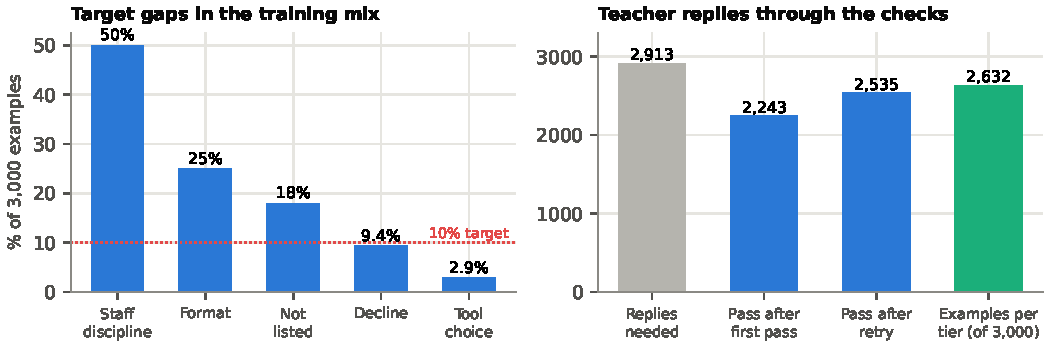
\includegraphics[width=0.95\textwidth]{figs/fig_data.pdf}
\caption{Left: share of the 3,000 examples per tier that carry each target gap (67\% are ordinary turns; an example can
carry more than one gap). Right: teacher replies through the checks, and the examples kept per tier.}
\label{fig:data}
\end{figure}

\subsection{Step 3: teacher replies, checks and hand review}
The oracle's drafts are correct but stilted, so a larger open model, Qwen3.5-9B (8-bit), rewrote each customer-facing reply
from the question, the shown information, the tool results, the correct action and the draft, keeping every fact, code and
price. It ran with llama.cpp on two T4s. \emph{Deviation:} the budget rule asked for a 27B pilot first; to keep GPU hours
in reserve the 9B was chosen before any GPU run. One reply serves both tiers (2,913 distinct replies).

Automatic checks, fixed before the run, drop a reply that is too long, contains tool-call markup, has an unsupported
detail (the run-time answer check), misses a required fact, drops a code or price, flips a yes/no or stock answer, lacks a
decline phrase where one is needed, offers staff on an answer, promises staff without a staff call, or is in the wrong
language. A stratified sample of 200 kept replies was then reviewed against the same rules, with the rule that more
than 10\% rejected tightens the checks.

The first pass kept 2,243 replies, and the review rejected 23 of 200 (11.5\%): 20 ended an answer with an offer to call
staff, mostly in Hinglish phrasings the offer pattern missed --- the very habit the 2B was being trained out of. The checks
were tightened (any staff mention on a non-staff action is rejected), each rejected reply was retried once with the
reason, and the sample was redrawn: 9 of 200 rejected (4.5\%), within the bar. The result is 2,632 examples per tier;
most of the dropped examples are near-miss ``no'' answers, so the decline share falls further below its floor.

\subsection{Step 4: training}
LoRA adapters of rank~16 ($\alpha = 32$, no dropout) were trained with Unsloth~\cite{unsloth} on the attention and MLP
projections of the language layers (Qwen3.5's linear-attention layers name their projections differently and were left
untouched), with loss on the model's own turns only: learning rate $2\times10^{-4}$ with cosine decay, effective batch 16,
8-bit AdamW, maximum length 4,096 tokens, seed 3407, and a 5\% held-out slice as a sanity check. The same settings trained
the 2B as QLoRA on a 4-bit base.
\begin{itemize}
  \item \emph{Deviation, before any training step.} The installed library no longer accepts a warm-up ratio, so the 5\%
        warm-up was given as a step count.
  \item \emph{Deviation after the smoke run.} A first reading suggested fp32 training, which would not fit the 4B on a
        T4; the second smoke run showed all three adapters loading in fp16 with finite losses, so the 4B stayed 16-bit
        LoRA as pre-registered. Two epochs would have taken 10--11 GPU hours, so each adapter was trained for
        \textbf{one epoch} (about 157 steps; two were pre-registered).
\end{itemize}
Full run: \placeholder{steps, minutes and final held-out loss per adapter: lora\_2b, qlora\_2b, lora\_4b}. The held-out
loss is a sanity check only; Step~6 decides.

\subsection{Step 5: the adapter on the deployed file}
Each adapter was converted to a GGUF adapter file with the converter from the same llama.cpp build as the laptop's server,
and loaded at run time next to its tier's deployed model file (2B Q8\_0, 4B Q4\_K\_M), not merged. Three rules had to hold
(Table~\ref{tab:step5}): the file loads with no error; the prompt the server builds from the harness's request matches the
training prompt on at least 95\% of 40 examples; and with the adapter at scale~0, greedy replies match plain decoding at least
as often as plain decoding matches itself. All three adapters passed every rule.

\begin{table}[H]
\centering\small
\caption{Step 5: loading the adapters on the deployed files.}\label{tab:step5}
\begin{tabular}{lrcccc}
\toprule
Adapter & Size & Loads & Template (rule $\ge$95\%) & Scale 0 vs plain & Ends turns (scale 1) \\
\midrule
lora\_2b & 21.8\,MB & yes & 40/40 & 8/8 (plain 8/8) & 8/8 \\
qlora\_2b & 21.8\,MB & yes & 40/40 & 8/8 (plain 8/8) & 8/8 \\
lora\_4b & 42.5\,MB & yes & 40/40 & 8/8 (plain 8/8) & 8/8 \\
\bottomrule
\end{tabular}
\end{table}

\subsection{Steps 6 to 8: deciding on dev}
\paragraph{Step 6, dev comparison.} Twenty runs on the laptop's GPU: O3-final, + lora\_2b and + qlora\_2b for Tier~A,
O3-final and + lora\_4b for Tier~B, each on 135 checked store questions, 60 tool cases, 60 follow-ups and 40 simulated
shopping dialogues. Each adapter run differs from its baseline only by the adapter, and the baselines were re-run in the same
plan. Tier~A carries lora\_2b to Step~7 if it is kept, otherwise qlora\_2b if kept and not worse than LoRA.

\paragraph{Step 7, patches removed.} ``Patches off'' means forced-answer recovery off (a printed call becomes the fixed
staff line and still counts as printed) and the staff check off; the staff guard is already off in O3-final. The entity
check, answer check and fallback are safeguards, not behaviour patches, and stay on. Runs: the Tier~A adapter with patches
off; the Tier~B adapter with the short-reply rule (40/60 words, 120 tokens); and the same with patches off. Two controls are
reported only: O3-final with patches off, and the 4B with short replies and no adapter. The result is a deployed candidate
per tier.

\paragraph{Step 8, speed and RAM.} Tier~A in place: the 2B on the laptop CPU with 4 threads, the 70-case dev speed subset,
two alternating repeats, for O3-final, O3-final + adapter, and the Step~7 candidate. The Tier~A adapter is deployed only
if both speed rules hold. Tier~B is reported from its Vulkan quality runs, which come from separate sittings and are
indicative only.

% ===========================================================================
\section{Results}\label{sec:results}
% ===========================================================================

\subsection{Step 6: all three adapters kept}
Figure~\ref{fig:step6} and Table~\ref{tab:step6} give the dev comparison. No set is worse for any adapter, the dialogues
stay at 100\% fit with one model request each, and pooled Hinglish does not fall (2B LoRA 82.6\% $\to$ 82.6\%, 2B QLoRA
$\to$ 89.1\%, 4B 84.8\% $\to$ 89.1\%).

\begin{figure}[H]
\centering
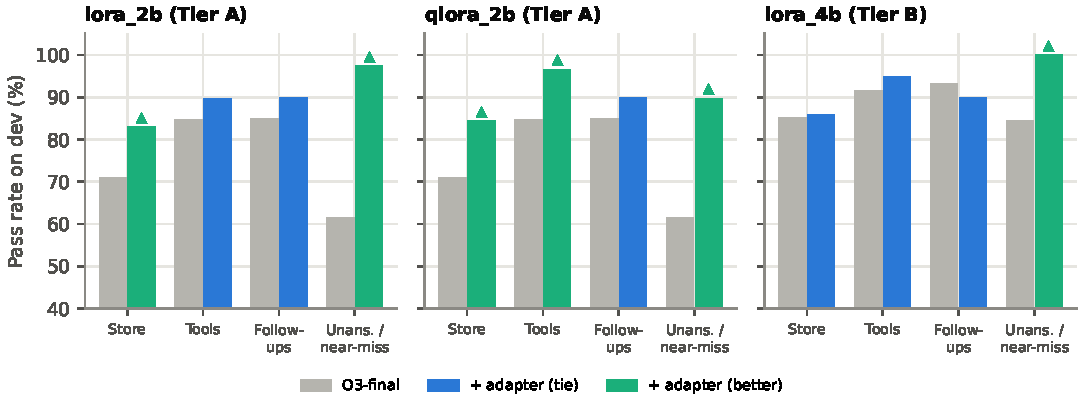
\includegraphics[width=\textwidth]{figs/fig_step6.pdf}
\caption{Dev pass rates, O3-final against O3-final with each adapter (Vulkan, paired). Green: better by the dev rule.}
\label{fig:step6}
\end{figure}

\begin{table}[H]
\centering\small
\caption{Step 6 sets on dev (difference in points, paired bootstrap 95\% interval).}\label{tab:step6}
\begin{tabular}{llrrrll}
\toprule
Adapter & Set & Cases & O3-final & + adapter & Difference [95\% CI] & Verdict \\
\midrule
lora\_2b & Store questions & 135 & 71.1\% & 83.0\% & +11.9 [+4.4, +19.3] & better \\
lora\_2b & Tool cases & 59 & 84.7\% & 89.8\% & +5.1 [$-$6.8, +15.3] & tie \\
lora\_2b & Follow-ups & 60 & 85.0\% & 90.0\% & +5.0 [$-$1.7, +13.3] & tie \\
qlora\_2b & Store questions & 135 & 71.1\% & 84.4\% & +13.3 [+5.9, +20.7] & better \\
qlora\_2b & Tool cases & 59 & 84.7\% & 96.6\% & +11.9 [+1.7, +22.0] & better \\
qlora\_2b & Follow-ups & 60 & 85.0\% & 90.0\% & +5.0 [$-$1.7, +13.3] & tie \\
lora\_4b & Store questions & 135 & 85.2\% & 85.9\% & +0.7 [$-$5.2, +7.4] & tie \\
lora\_4b & Tool cases & 60 & 91.7\% & 95.0\% & +3.3 [0.0, +8.3] & tie \\
lora\_4b & Follow-ups & 60 & 93.3\% & 90.0\% & $-$3.3 [$-$11.7, +5.0] & tie \\
\bottomrule
\end{tabular}
\end{table}

\paragraph{The hypotheses.} Figure~\ref{fig:behaviour} shows the behaviour the adapters were trained for.
\begin{itemize}
  \item \textbf{H1 holds for both models.} Printed tool calls fall to zero in every set: 3 $\to$ 0 on the 2B's store
        questions and 3 $\to$ 0 on the 4B's follow-ups.
  \item \textbf{H2 holds.} The 2B's own staff calls on answerable store questions fall from 20 to 0, with answerable
        questions a tie (75.0\% $\to$ 77.1\%).
  \item \textbf{H3 holds.} The 2B's unanswerable and near-miss questions rise from 61.5\% to 97.4\% (+35.9 [+20.5, +51.3]),
        and replies with an unsupported detail fall from 8 of 130 to 2 of 131. The 4B, not tested on H3, rises from 84.6\%
        to 100\%.
  \item \textbf{H6 goes against the expectation.} QLoRA is not worse than LoRA on any set and better on tool cases
        (+6.7 [+1.7, +13.3]). The carry rule takes lora\_2b because it was kept; QLoRA's result is recorded for the final
        round.
\end{itemize}

\begin{figure}[H]
\centering
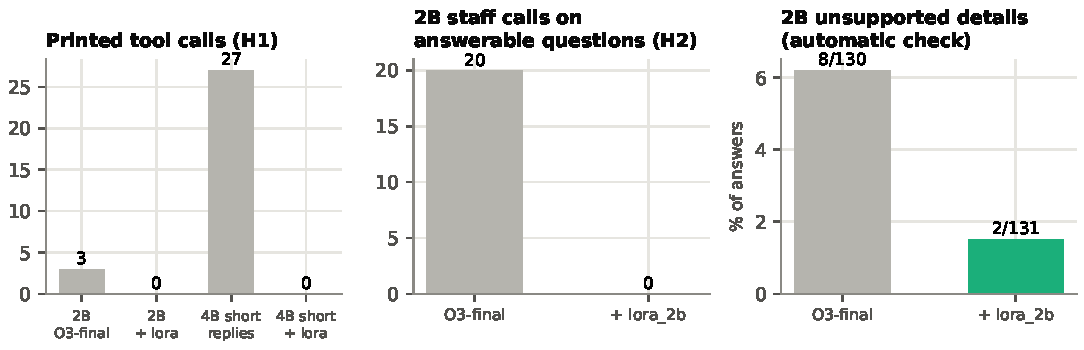
\includegraphics[width=0.95\textwidth]{figs/fig_behaviour.pdf}
\caption{The trained behaviour on dev. Left: printed tool calls (2B: store questions; 4B: all sets with the short-reply
rule, without the adapter as the control, Step~7). Middle and right: the 2B's staff calls on answerable questions, and its
replies with a detail found in no shown card or tool result.}
\label{fig:behaviour}
\end{figure}

\paragraph{Why the 2B got faster.} With the adapter the 2B answers store questions in 0.87 model rounds instead of 2.01,
reads 312 tokens before answering instead of 433, and no longer calls tools it does not need; on the GPU its median first
word on store questions fell from 5.5\,s to 2.1\,s. Kiosk time per shopping dialogue fell from 9.9 to 8.5\,s.

\subsection{Step 7: the patches can go}
Figure~\ref{fig:step7} and Table~\ref{tab:step7} give the patch removal.
\begin{itemize}
  \item \textbf{Tier~A, H5 holds.} lora\_2b with the patches off is better on store questions (+11.9) and ties elsewhere,
        with no printed call. Without the adapter, switching the patches off prints 14 tool calls (12 on store
        questions), so the patches were doing real work that the adapter now does.
  \item \textbf{Tier~B, the short replies return.} Without the adapter, the 4B with short replies is worse on store
        questions ($-$9.0) and tool cases ($-$8.3) and prints 27 tool calls; with lora\_4b it ties everywhere and prints
        none, with the patches on or off. H5 holds for Tier~B too.
\end{itemize}
The deployed candidates for Step~8 are therefore O3-final + lora\_2b with the patches off (Tier~A), and O3-final + lora\_4b
with short replies and the patches off (Tier~B).

\begin{figure}[H]
\centering
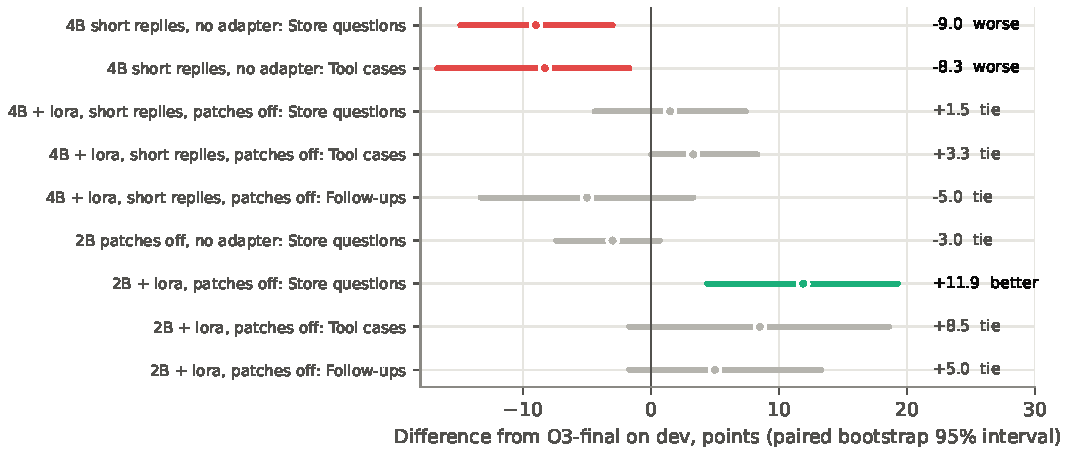
\includegraphics[width=0.95\textwidth]{figs/fig_step7.pdf}
\caption{Step 7 on dev: each run against O3-final. The two runs without an adapter are controls, reported only.}
\label{fig:step7}
\end{figure}

\begin{table}[H]
\centering\small
\caption{Step 7: no regression, and printed tool calls (store / tool cases / follow-ups / dialogues).}\label{tab:step7}
\begin{tabularx}{\textwidth}{L lll c c}
\toprule
Run & Store & Tools & Follow-ups & Printed & Holds \\
\midrule
lora\_2b, patches off & better & tie & tie & 0/0/0/0 & yes \\
O3-final 2B, patches off (control) & tie & tie & tie & 12/0/2/0 & no \\
lora\_4b, short replies & tie & tie & tie & 0/0/0/0 & yes \\
lora\_4b, short replies, patches off & tie & tie & tie & 0/0/0/0 & yes \\
O3-final 4B, short replies (control) & worse & worse & tie & 14/6/5/2 & no \\
\bottomrule
\end{tabularx}
\end{table}

\subsection{Step 8: speed and RAM}\label{sec:speed}
Table~\ref{tab:step8} and Figure~\ref{fig:step8} give the in-place timing on the laptop CPU.

\begin{table}[H]
\centering\small
\caption{Step 8, Tier~A in place (2B Q8\_0, CPU, 4 threads, 70 dev cases, 2 repeats).}\label{tab:step8}
\begin{tabularx}{\textwidth}{p{2.4cm} L L L}
\toprule
Set & Writing speed, tokens/s (rule 1: $\ge$90\%) & Total time, candidate (rule 2) & First word, candidate \\
\midrule
Store questions & 16.1 $\to$ 15.4 (96\%) \met & $-$2.01\,s [$-$5.80, $-$0.40] \met & $-$2.24\,s [$-$5.96, $-$0.06] \\
Tool cases & 15.1 $\to$ 14.6 (96\%) \met & +2.65\,s [+0.01, +4.17] \missed & +3.31\,s [+0.01, +3.97] \\
\bottomrule
\end{tabularx}
\end{table}

\begin{figure}[H]
\centering
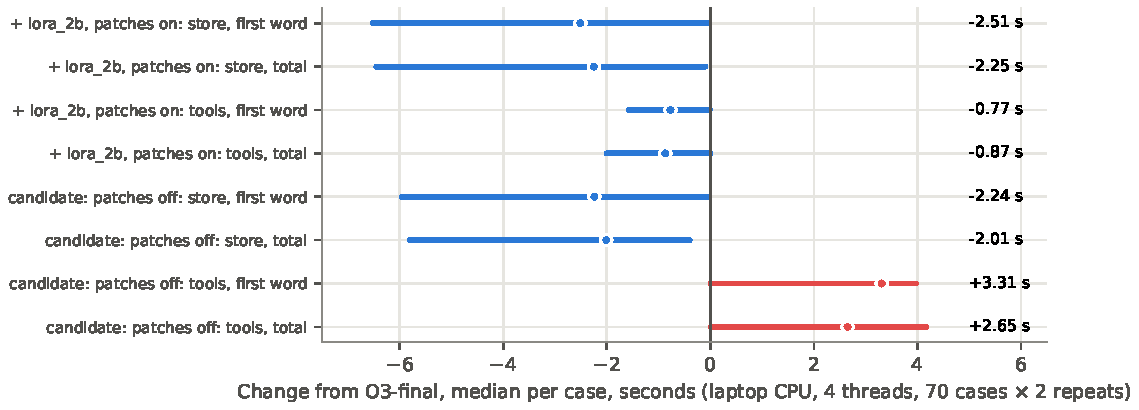
\includegraphics[width=0.95\textwidth]{figs/fig_step8.pdf}
\caption{Tier~A in place: median per-case change from O3-final, with bootstrap 95\% intervals. Red: significantly longer.}
\label{fig:step8}
\end{figure}

\begin{itemize}
  \item \textbf{The adapter's own cost is small.} Writing speed keeps 96\% of O3-final's on both sets (rule~1), and peak
        server memory is 2,304\,MB against 2,433\,MB, within the expected 0.2\,GB.
  \item \textbf{The candidate fails rule 2 on tool cases.} With the patches off, the 2B's tool-case replies take 2.65\,s
        longer at the median, and the interval just excludes zero (+0.01\,s). On store questions the candidate is
        2.0\,s faster. In this run the patches-off configuration read more tokens before answering on tool cases (209
        against 161) with the same quality; the cause was not investigated, and the same comparison was not run in a
        second sitting.
  \item \textbf{By the rule, Tier~A keeps O3-final.} The adapter's quality gain is reported with its speed cost.
  \item \textbf{Reported, not deciding.} The same adapter with the patches on was faster than O3-final on both sets in
        the same sitting (store questions $-$2.25\,s, tool cases $-$0.87\,s) and would have met both rules. It was not the
        Step~7 candidate, so choosing it now would be choosing after seeing the result; it is the configuration to confirm
        first in the final round.
\end{itemize}

\paragraph{Tier B (indicative).} From the Vulkan quality runs, the deployed Tier~B candidate writes at 91\% of
O3-final's speed (9.7 $\to$ 8.8 tokens/s on store questions), its first word comes 0.2--0.8\,s later, and its total reply
time is 0.9\,s shorter on store questions, 0.2\,s shorter on tool cases and 1.3\,s longer on follow-ups.

\subsection{What the adapters got wrong}\label{sec:failures}
A review of every dev case that changed found three costs the set verdicts do not show.
\begin{enumerate}
  \item \textbf{Declining answerable store questions.} Both adapters now decline some policy and care questions whose
        answer was shown: the 4B lost transfers from another branch, gift receipts, an automatic's power reserve,
        working out, steam rooms and cleaning after the beach (answerable questions 85.4\% $\to$ 81.2\%, a tie); the 2B
        lost a power-reserve question, gold plating and an engraving question in Hinglish. The training data's many
        ``I don't have that'' examples taught the decline a little too broadly.
  \item \textbf{Colour follow-ups (4B).} On ``does it come with a red dial?'' after a product, the 4B adapter answers ``not
        listed'' or ``no'' when the stock check showed that colour: 90\% $\to$ 50\% (40\% with patches off) on 10 cases,
        a subset reported as worse.
  \item \textbf{Staff promises.} The adapters now end many declines with an offer to call staff, asked as a question
        (2B: 11 $\to$ 39), as trained. In two 2B tool cases (one with the patches off) the reply said staff were coming
        without a staff call.
\end{enumerate}
None of these was fixed on dev: they are targets for the training data of the final round.

\subsection{Scorecard}
\begin{table}[H]
\centering\small
\caption{Objective 4 on dev, against O3-final.}\label{tab:score}
\begin{tabularx}{\textwidth}{L p{3.6cm} p{3.6cm}}
\toprule
Criterion & Tier A (2B) & Tier B (4B) \\
\midrule
Adapter kept (H4 and one of H1--H3) & lora\_2b and qlora\_2b \met & lora\_4b \met \\
H1, printed tool calls $\le 1$ per set & 0 in every set \met & 0 in every set \met \\
H2, staff calls on answerable halved & 20 $\to$ 0 \met & -- \\
H3, declines +5 points & +35.9 \met & -- (+15.4 reported) \\
H4, no regression & no set worse \met & no set worse \met \\
H5, patches off & holds \met & holds, with short replies \met \\
H6, QLoRA not better than LoRA & better on tool cases (against expectation) & -- \\
Speed rule 1, writing speed $\ge$90\% & 96\% \met & 91\% (reported) \\
Speed rule 2, total time not longer & tool cases +2.65\,s \missed & -- (reported) \\
RAM, under +0.2\,GB & $-$0.13\,GB \met & -- \\
\midrule
Deployed & O3-final (no adapter) & O3-final + lora\_4b, short replies, patches off \\
\bottomrule
\end{tabularx}
\end{table}

% ===========================================================================
\section{Decisions and reasoning}\label{sec:decisions}
% ===========================================================================
{\small
\begin{xltabular}{\textwidth}{>{\raggedright\arraybackslash}p{3.6cm} >{\raggedright\arraybackslash}p{4.4cm} L}
\caption{Decision log.}\label{tab:decisions}\\
\toprule
Decision & Evidence & Reasoning \\
\midrule
\endfirsthead
\toprule Decision & Evidence & Reasoning \\ \midrule \endhead
Train behaviour, keep facts in retrieval & Facts change with the catalogue & An adapter trained on facts would go stale with
every catalogue update. \\
A disjoint training catalogue & No shared name, style or code & The adapter cannot memorise the store; any gain is
behaviour. \\
Code decides every action & The oracle runs O3-final's own harness & Labels are correct by construction, and training text
equals run-time text. \\
Run-time adapter, route (a) & Loads on the deployed file; scale 0 matches plain decoding 8/8 & The deployed weights stay
byte-identical, and an adapter can be switched off per request. \\
Teacher 9B without a 27B pilot (deviation) & 20-hour GPU budget & Decided before any GPU run; the hand review (4.5\%
rejected) shows the 9B was adequate. \\
Tighten checks after 11.5\% rejected & 20 of 23 rejects offered staff & The pre-registered rule; it removed the habit being
trained out. \\
One epoch, not two (deviation) & Two epochs: 10--11 GPU hours & Decided after the smoke run, before the full run. \\
Carry lora\_2b, not qlora\_2b & lora\_2b kept & The pre-registered carry rule; QLoRA's tool-case gain is recorded. \\
Patches off for both tiers & H5 holds; controls print 14 and 27 calls & The adapters do what the patches did. \\
Tier~A stays O3-final & Speed rule 2 missed on tool cases & The pre-registered rule; patches-on is not chosen after the
fact. \\
Tier~B: lora\_4b, short replies, patches off & Short-reply check and H5 hold & Recovers the 4B's short replies, the
main prize expected for Tier~B. \\
Do not fix the over-declining on dev & Found in the case review & Fixing it on dev would tune on dev; it goes into the
final round's data. \\
\bottomrule
\end{xltabular}}

% ===========================================================================
\section{Limitations and threats to validity}\label{sec:limits}
% ===========================================================================
\begin{itemize}
  \item \textbf{Dev data only.} By design this round has no test set: the Objective~4 test set is built with the company's
        data and used once. The dev sets also shaped Objective~3's harness, so the gains here may be optimistic.
  \item \textbf{No judged hallucination.} The blind judge of Objective~3 was not re-run, so the adapters' effect on
        judged unsupported claims is unknown; the automatic check (8 $\to$ 2 of 130 for the 2B) sees only checkable
        details.
  \item \textbf{Fictional data and a smaller teacher.} The training catalogue, questions and dialogues are generated, and
        the replies come from a 9B teacher. Decline and tool-choice examples fell below their 10\% floor.
  \item \textbf{One epoch.} The adapters saw their data once, half the pre-registered schedule.
  \item \textbf{Small subsets.} Follow-up types have 10 cases each and Hinglish subsets 10--22, so one case moves them by
        5--10 points; only the pooled Hinglish check decides.
  \item \textbf{Timing.} Tier~A's decisive timing is one sitting with two repeats, and the failing interval's lower bound
        is +0.01\,s. Tier~B's timings come from separate sittings and are indicative only.
\end{itemize}

% ===========================================================================
\section{Next steps: the final round}\label{sec:next}
% ===========================================================================
When the company's data arrives, the same pipeline is run once more, with these changes:
\begin{itemize}
  \item \textbf{Data.} More answer examples for policy, care and colour-variant questions whose answer is shown, so the
        decline is learned only where it applies; staff promises only with a staff call; decline and tool-choice shares at
        their floor.
  \item \textbf{Training.} The pre-registered two epochs; QLoRA kept in the comparison, given its tool-case result.
  \item \textbf{Tier~A configuration.} The 2B adapter with the patches on is the first candidate, with the speed rules
        checked in two sittings.
  \item \textbf{Route (b).} Merged and re-quantised weights against the run-time adapter, with a control model put through
        the same conversion without training.
  \item \textbf{Evaluation.} A fresh Objective~4 test set from the Objective~3 builder with new seeds, used once, and the
        blind judge re-run on the deployed candidates.
\end{itemize}

\begin{thebibliography}{99}
\bibitem{lora} E.~J.~Hu et al. LoRA: Low-rank adaptation of large language models. \emph{ICLR}, 2022.
\bibitem{qlora} T.~Dettmers, A.~Pagnoni, A.~Holtzman, L.~Zettlemoyer. QLoRA: Efficient finetuning of quantized LLMs.
  \emph{NeurIPS}, 2023.
\bibitem{unsloth} D.~Han, M.~Han and contributors. \emph{Unsloth}. Open-source software,
  \url{https://github.com/unslothai/unsloth}.
\bibitem{llamacpp} G.~Gerganov and contributors. \emph{llama.cpp: LLM inference in C/C++}. Open-source software,
  \url{https://github.com/ggml-org/llama.cpp}.
\bibitem{efron} B.~Efron and R.~J.~Tibshirani. \emph{An Introduction to the Bootstrap}. Chapman \& Hall, 1993.
\bibitem{mcnemar} Q.~McNemar. Note on the sampling error of the difference between correlated proportions or
  percentages. \emph{Psychometrika}, 12(2):153--157, 1947.
\end{thebibliography}

\appendix
\section{Adapter and training settings}\label{app:config}
\begin{small}
\begin{tabularx}{\textwidth}{l L}
\toprule
Setting & Value \\
\midrule
Base weights & 16-bit originals of the deployed files (Qwen3.5-2B, Qwen3.5-4B); QLoRA on a 4-bit 2B base \\
Adapter & LoRA rank 16, $\alpha = 32$, dropout 0; q, k, v, o, gate, up, down projections of the full-attention and MLP
layers; vision layers untouched \\
Optimisation & learning rate $2\times10^{-4}$, cosine decay, 5\% warm-up (as steps), effective batch 16, 8-bit AdamW, no
weight decay, fp16 mixed precision, seed 3407, 1 epoch (deviation from 2) \\
Data & 3,000 planned and 2,632 kept examples per tier; loss on the answer only; maximum 4,096 tokens; 5\% held out by
question id \\
Teacher & Qwen3.5-9B Q8\_0, llama.cpp, 2 $\times$ T4, temperature 0.7 with a seed per reply, thinking off; word limits 40
(fact), 60 (recommendation), 35 (rephrased fixed reply) \\
Run time & adapter GGUF (f16) loaded next to the deployed GGUF by llama-server; scale set per request \\
Deployed Tier~B & O3-final + lora\_4b, short replies (40/60 words, 120 tokens), forced-answer recovery and staff check off \\
Hardware & Intel Core i5-1240P, 16\,GB RAM, Intel Iris Xe graphics (runs); 2 $\times$ NVIDIA T4 (teacher, training) \\
\bottomrule
\end{tabularx}
\end{small}

\end{document}
